\section{How it works}
This section describes how self-propelled instrumentation works in details.
Each subsection is a major step in the workflow.
Thw workflow is visualized in Figure~\ref{fig:workflow}.

% The workflow:
% 1. injector hijacks a process
% 2. agent is loaded in the process
% 3. init function in agent is executed
%   3.1 register event
%   3.2 register payload function
%   3.3 other configuration
% 4. event activation, doing initial instrumentation
% 5. propagation

\begin{figure}[ht]
  \centering
  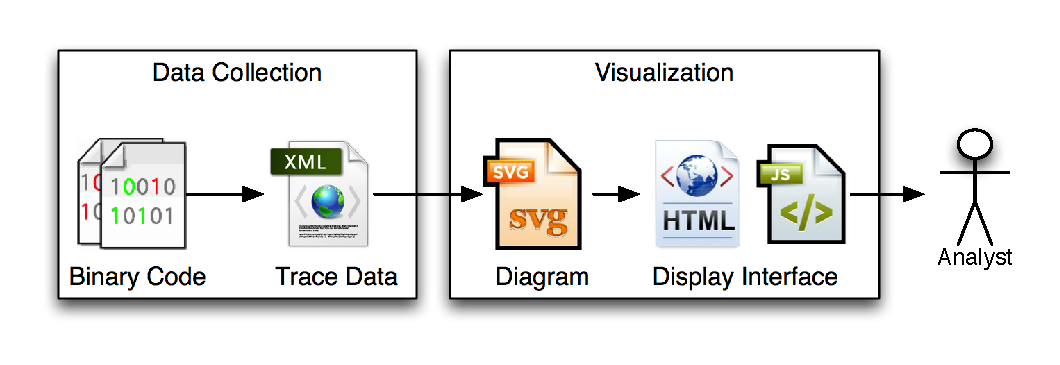
\includegraphics[width=0.70\textwidth]{figure/workflow.eps} 
  \caption{Self-propelled Instrumentation Workflow} \label{fig:workflow}
\end{figure}

\subsection{Building Agent}
Users build their own {\em Agent} shared library using self-propelled
instrumentation's API.
\begin{enumerate}
\item Coding. Users need to write two pieces of code: 1) payload function; 2)
  configuration code that registers payload function and does some customization
  and configuration. The configuration code must be executed right away when the
  {\em Agent} shared library is loaded into the application process, so the
  configuration code should be in the init function of the {\em Agent} shared
  library, i.e., the function with gcc directive
  \_\_attribute\_\_((constructor)).
\item Building. Users build the code into an {\em Agent} shared library linking
  with {\em libagent.so} provided by the self-propelled instrumentation
  infrastructure.
\end{enumerate}

\subsection{Injection}
Users run {\em Injector} in command line. They specify in command line arguments
the path of an {\em Agent} shared library and the application process to inject
to.

One trick to check whether the {\em Agent} shared library is injected
successfully is to look at memory maps file of the application process, i.e.,
/proc/PID/maps.

\subsection{Configuration}
The configuration code is executed right away when {\em Agent} shared library is
load into the application process.
It tells self-propelled instrumentation what are payload functions provided by
users, how would initial instrumentation be done, whether or not to enable
inter-process instrumentation propagation ...

\subsection{Initial Instrumentation}

\subsection{Intra-process Propagation}

\subsection{Inter-process Propagation}
